\section{Risultati e discussione finale}\label{sec:risultati}
\normalsize

Per trarre le conclusioni di questo studio useremo i risultati delle metriche e dei tempi di addestramento. Questi ci permetteranno di capire quale modello è migliore in quali circostanze, certi scenari traggono maggior vantaggio dalla leggerezza del modello, mentre altri prediligono la precisione nelle predizioni.\\*\\*
Il grafico seguente contiene i risultati di tutti i modelli e lo loro versioni, divisi secondo le metriche scelte.
\begin{figure}[ht]
	\makebox[\textwidth][c]{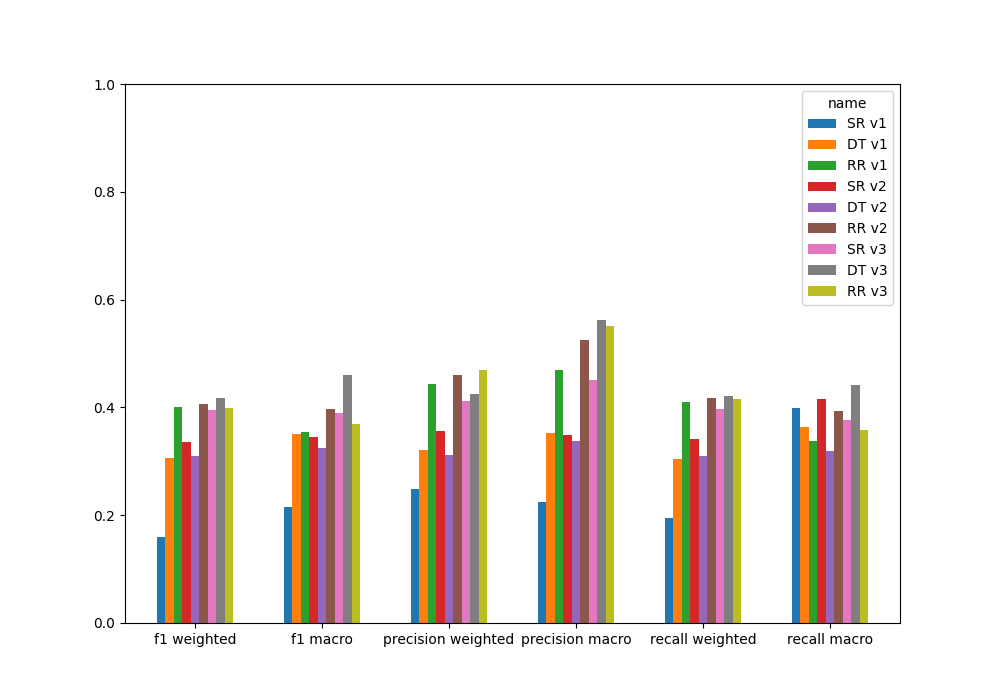
\includegraphics[scale=0.8]{../figures/results.PNG}}
	\caption{Grafico risultati}
	\label{fig:ris}
\end{figure}


Come si può vedere non tutti i modelli sono migliorati con il pre-processing dei dati e l'implementazione delle versioni in ensemble, ma forse la sorpresa più grossa sono le prestazioni del modello di Ridge regression, che anche nella sua versione più semplice ha ottenuto risultati paragonabili alle versioni in ensemble degli altri modelli.\\*\\*
Oltre alle metriche valuteremo anche i tempi di addestramento di ogni modello, che per comodità sono stati riportati nel grafico sotto.

\begin{figure}[htp]
	\makebox[\textwidth][c]{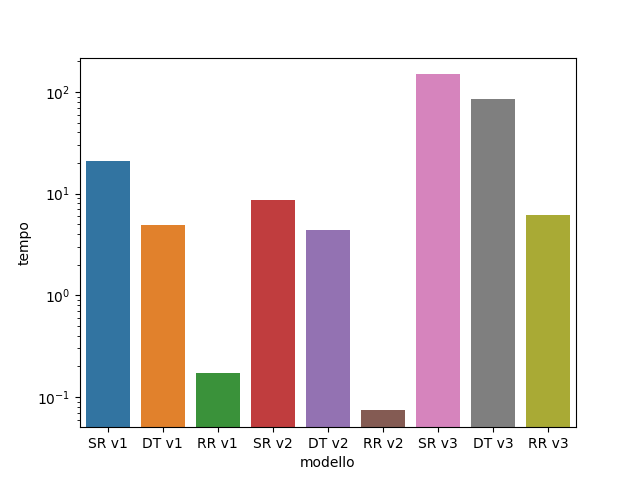
\includegraphics[scale=0.8]{../figures/timings.PNG}}
	\caption{Grafico tempi di addestramento}
	\label{fig:times}
\end{figure}

\subsection{Risultati della Softmax regression}\label{ssec:softmaxRes}
\normalsize
Questo modello è stato selezionato per essere una base line, ovvero un termine di paragone, e si è comportato esattamente come ci aspettavamo.\\*\\*
Nella versione 1, quella basilare con i dati originali, ha avuto risultati abbastanza scadenti e incostanti, spesso ha mostrato anche segni di Overfitting, il suo f1 score weighted oscilla solitamente tra lo 0.1 e lo 0.2, ma penso che il dato più critico sia che spesso non riesce a predire nessun elemento di alcune classi. Questa è una grossa criticità che non è possibile ignorare.\\*\\*
Nella versione 2, che usa lo stesso modello della prima, ma con i dati pre-processati, i risultati sono tendenzialmente migliori, l’f1 score weighted in questo caso si aggira spesso attorno allo 0.3 e raramente scende sotto lo o.25, in più non sembra più soffrire di overfitting. Questo è un progresso non da poco, ma rimane comunque il problema che a volte non riesce a classificare certe classi, anche se è diventato un evento più raro rispetto a prima.\\*\\*
Nella versione 3, che usa un ensemble con i dati pre-processati, finalmente si raggiungono dei risultati accettabili. L'f1-score weighted purtroppo resta sempre attorno a 0.4, ma è comunque un progresso rispetto a prima, l'incapacità di riconoscere certe classi è diventa un'eventualità molto rara in questa versione.\\*\\*
I risultati di questo modello sono buoni, ma i tempi di addestramento della Softmax regression sono i più alti se si paragonano alle stesse versioni degli altri modelli.\\*\\*
Comunque abbiamo ottenuto ciò che volevamo da questo modello, siamo riusciti a dimostrare l’efficacia che tecniche come pre-processing ed ensemble possono avere su certi algoritmi e ora abbiamo una buona base da paragonare agli altri algoritmi per evidenziarne gli effettivi pregi.
\subsection{Risultati della Decision tree classificator}\label{ssec:DecisionRes}
\normalsize
Questo modello è stato scelto principalmente per avere la sua versione in ensamble, ma anche la sua versione più semplice ha dimostrato una buona performance.\\*\\*
Nella versione 1 questo algoritmo ha avuto risultati paragonabili alla versione 2 della softmax regression, ma non ha avuto grandi miglioramenti una volta aggiornato alla versione 2, anzi le performance sono leggermente inferiori. \\*\\*
Ciò sottolinea che un classificatore basato su Decision tree non ha grossi problemi con dati non pre-processati, che è un punto a favore visto che è una cosa in meno da fare.\\*\\*
In più vorrei sottolineare che questo modello riesce sempre a classificare almeno una parte dei campioni per ciascuna classe anche nelle versioni 1 e 2, quindi non ha il problema principale che penalizzava la Softmax regression.\\*\\*
La sua versione 3 invece ha risultati paragonabili a quelli dell’ensemble della Softmax regression, ma in media il tempo impiegato per addestrare il modello dell’algoritmo è la metà.\\*\\*
Tirando le somme nel confronto tra Softmax regression e Decision tree, il secondo risulta superiore sotto ogni aspetto, riesce ad ottenere prestazioni paragonabili alla Softmax regression con pre-processing anche nella sua versione più semplice e lo fa impiegando meno tempo, quindi si può dire che la versione 1 del Decision tree è migliore delle prime due versioni della Softmax regression e anche la terza si comporta meglio della corrispettiva ottenendo gli stessi risultati in meno tempo.\\*\\*

\subsection{Risultati della Ridge regression}\label{ssec:DecisionRes}
\normalsize
Questo ultimo modello è quello che mi ha sorpreso di più durante questa analisi. Pur essendo uno strumento usato nella regressione, ovvero nella previsione di valori continui, è riuscito ad ottenere ottime prestazioni anche in un caso di classificazione. \\*\\*
In più la sua caratteristica di essere un modello di regressione ci permette di calcolare il mean square error in modo facile e capire di conseguenza di quanto si sbagliano le classificazioni errate, permettendoci di valutare l'utilità del modello in caso la sua precisione non sia alta.\\*\\*
I risultati della versione 1 di questo modello sono i più sorprendenti, senza pre-preprocessing o ensemble riesce a ottenere delle prestazioni paragonabili, e spesso anche superiori, rispetto ai modelli in ensemble delle altre due alternative. Anche se comunque l’f1 score weighted resta spesso vicino allo 0.4 e non supera mai lo 0.5, quindi in generale non ha dei punteggi altissimi.\\*\\*
Il suo aspetto migliore sono i tempi di addestramento! Se confrontato alle versioni migliori degli altri due modelli, il paragone è schiacciante: i tempi di addestramento della ridge regression sono circa 2 decimi di secondo, mentre Softmax regression e Random forest classifier impiegano rispettivamente circa 150 e 80 secondi.\\*\\*
La  versioni 2 è leggermente più precisa della versione 1 e impiega ancora meno tempo per l'addestramento, meno di 1 decimo di secondo.\\*\\*
Diversamente la versione 3 non è molto conveniente, finisce con l'avere dei risultati leggermente migliori, ma scambiandoli per tempi di addestramento molto più lunghi, anche se comunque migliori delle stesse versioni degli altri modelli.\\*\\*
L'ultima nota è che il mean square error dell’algoritmo è sempre circa 1, che vuol dire che anche quando la predizione è errata il suo valore è solitamente nelle classi adiacenti a quella corretta. Per questo è possibile trovare alcune applicazioni pratiche anche se la precisione dell'algoritmo non è altissima.\\*\\*
Tirando le conclusioni, la Ridge regression risulta il modello migliore perché ottiene le prestazioni più alte con un tempo di addestramento molto inferiore. La sua versione migliore risulta essere la versione 2, dimostrando nuovamente l'utilità del pre-processing in questo ambito. Queste sue caratteristiche lo rendono sicuramente il modello migliore per provare future applicazioni in campo reale, in particolare i suoi tempi di addestramento molto veloci permettono a questo modello di essere scalato con molti più campioni e mantenere comunque dei tempi di risposta di tutto rispetto.\\*\\*
\subsection{Considerazioni finali e futuri sviluppi}\label{ssec:DecisionRes}
\normalsize
In molti videogiochi i giocatori sono divisi in leghe o gradi in base a un sistema a punti, come già accennato nell'introduzione, tale sistema funziona molto bene per la maggior parte dei giocatori, che avendo una crescita graduale riescono a migliorare nel tempo e crescere conseguentemente di livello.\\*\\*
Però penso che questo sistema non riesca a individuare bene le anomalie, ovvero i giocatori che hanno un livello di partenza molto alto. Alcuni giochi, Starcraft compreso, hanno un sistema di piazzamento iniziale, dove viene chiesto al giocatore di giocare alcune partite per essere piazzato al grado corretto. Questa modalità riesce a catturare alcune di queste anomalie, ma non sempre è efficacie, nei sistemi a punti spesso una volta posizionati in una lega ci vuole del tempo per poter scalare i vari gradi.\\*\\*
Ad esempio, un giocatore potrebbe giocare male di proposito nelle 10-15 partite di piazzamento per poi usare l'account per fare Smurfing, fenomeno sempre più diffuso nel mondo dei videogiochi che peggiora l'esperienza videoludica di molti giocatori alle prime armi.\\*\\*
I risultati di questo studio dimostrano che la classificazione fatta usando tecniche di machine learning potrebbe essere una buona opzione in questo ambito. Sicuramente sarà necessario risolvere alcune criticità, ma penso che queste tecnologie abbiano una prospettiva molto promettente nel mondo videoludico.